\section{Moment pędu}

\subsection{Momentu pędu w mechanice klasycznej}
W mechanice klasycznej moment pędu (inaczej moment kątowy) cząstki względem punktu odniesienia definiujemy jako iloczyn wektorowy położenia $\vec{r}$ i pędu $\vec{p}$
$$
\vec{L} = \vec{r} \times \vec{p}.
$$
\begin{figure}[H]
\centering
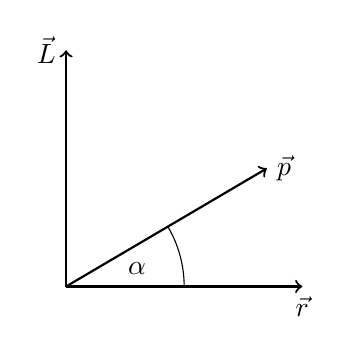
\begin{tikzpicture}[scale=1.5]
\begin{scope}
  \draw[->, thick] (0,0) -- (2,0) node[below] {$\vec{r}$};
  \draw[->, thick] (0,0) -- (0,2) node[left] {$\vec{L}$};
  \draw[->, thick] (0,0) -- (1.7,1) node[right] {$\vec{p}$};
  \draw (1,0) arc (0:30:1);
  \node at (0.6,0.15) {$\alpha$};
\end{scope}
\end{tikzpicture}
\caption{Moment pędu jako iloczyn wektorowy $\vec{r}$ i $\vec{p}$.}
\end{figure}

Wartość bezwzględna momentu pędu wynosi
$$
|\vec{L}| = |\vec{r}| \cdot |\vec{p}| \cdot \sin \alpha,
$$
gdzie $\alpha$ to kąt między wektorami $\vec{r}$ i $\vec{p}$. Moment pędu jest więc wielkością wektorową, prostopadłą do płaszczyzny rozpiętej przez $\vec{r}$ i $\vec{p}$.
\begin{figure}[H]
\centering
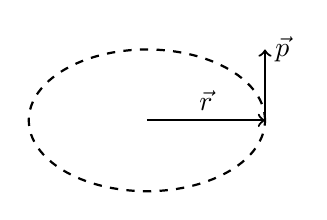
\begin{tikzpicture}[scale=1.5]
\begin{scope}
  \draw[dashed, thick] (0,0) ellipse (1 and 0.6);
  \draw[->, thick] (0,0) -- (1,0) node[midway, above] {$\vec{r}$};
  \draw[->, thick] (1,0) -- (1,0.6) node[right] {$\vec{p}$};
\end{scope}
\end{tikzpicture}
\caption{Moment pędu jako wektor prostopadły do płaszczyzny rozpiętej przez $\vec{r}$ i $\vec{p}$.}
\end{figure}

\subsubsection*{Zasada zachowania momentu pędu}
W układach \textbf{stacjonarnych}, czyli takich, w których nie zmieniają się parametry układu w czasie, zachodzi zasada zachowania momentu pędu
$$
\frac{d\vec{L}}{dt} = 0 \quad \Rightarrow \quad \vec{L} = \text{const.}
$$
Oznacza to, że moment pędu nie ulega zmianie w czasie, jeśli na układ nie działa moment sił zewnętrznych (np. brak momentu zewnętrznego lub centralna symetria pola).

Zachowanie całkowitego momentu pędu wynika z symetrii układu, a w szczególności z~\textbf{symetrii osiowej}. W języku mechaniki klasycznej mówi się wówczas, że jest to \textbf{całka ruchu}.

\subsection{Moment pędu w mechanice kwantowej}
W mechanice kwantowej moment pędu staje się \textbf{operatorem}. Składowe klasycznego momentu pędu można zapisać w postaci
$$
\begin{aligned}
L_x &= y p_z - z p_y, \\
L_y &= z p_x - x p_z, \\
L_z &= x p_y - y p_x.
\end{aligned}
$$

Po przejściu do przestrzeni operatorów (czyli do formalizmu mechaniki kwantowej), każdej z wielkości przypisujemy odpowiedni operator. Operatory składowych momentu pędu przyjmują postać
$$
\begin{aligned}
\hat{L}_x &= -i\hbar \left( y \frac{\partial}{\partial z} - z \frac{\partial}{\partial y} \right), \\
\hat{L}_y &= -i\hbar \left( z \frac{\partial}{\partial x} - x \frac{\partial}{\partial z} \right), \\
\hat{L}_z &= -i\hbar \left( x \frac{\partial}{\partial y} - y \frac{\partial}{\partial x} \right),
\end{aligned}
$$
gdzie $\hbar$ to zredukowana stała Plancka.

Operator momentu pędu jako wielkość wektorowa zapisuje się ogólnie w postaci
$$
\vec{\hat{L}} = -i\hbar\, \vec{r} \times \vec{\nabla},
$$
gdzie $\vec{r} = (x, y, z)$ jest operatorem położenia, a $\vec{\nabla} = \left( \frac{\partial}{\partial x}, \frac{\partial}{\partial y}, \frac{\partial}{\partial z} \right)$ jest operatorem gradientu.

\subsubsection*{Komutatory operatorów momentu pędu}
$$
\begin{aligned}
[L_x, L_y] &= [y p_z - z p_y, z p_x - x p_z] \\
&= [y p_z, z p_x] - [z p_y, z p_x] - [y p_z, x p_z] + [z p_y, x p_z]
\end{aligned}
$$

$$
[yp_z, zp_x] = yp_z zp_x - zp_x yp_z = y p_x [p_z, z] = -i\hbar y p_x
$$

Poniżej przedstawione są komutatory
$$
\begin{aligned}
  [\hat{L}_x, \hat{L}_y] &= i\hbar(xp_y - yp_x) = i \hbar \hat{L}_z, \\
  [\hat{L}_y, \hat{L}_z] &= i \hbar \hat{L}_x, \\
  [\hat{L}_z, \hat{L}_x] &= i \hbar \hat{L}_y.
\end{aligned}
$$
Z powyższych relacji wynika, że operatory składowych momentu pędu nie komutują ze sobą
$$
[\hat{L}_x, \hat{L}_y] \neq 0,
$$
co oznacza, że nie można jednocześnie znać dokładnych wartości wszystkich trzech składowych momentu pędu.

Gdyby nie operatory to poniższa relacja byłaby sprzeczna
$$
\hat{\vec{L}} \times \hat{\vec{L}} = i\hbar \hat{\vec{L}}.
$$

\subsubsection*{Operator $\hat{L}^2$}
Kwadrat całkowitego momentu pędu zdefiniowany jest jako
$$
\hat{L}^2 = \hat{L}_x^2 + \hat{L}_y^2 + \hat{L}_z^2.
$$
Działa on jako operator skalarowy. Co istotne, komutuje ze wszystkimi składowymi momentu pędu
$$
[\hat{L}^2, \hat{L}_x] = [\hat{L}^2, \hat{L}_y] = [\hat{L}^2, \hat{L}_z] = 0.
$$
Zatem można jednocześnie mierzyć $\hat{L}^2$ i jedną wybraną składową, np. $\hat{L}_z$.

\subsubsection*{Wybór układu współrzędnych -- baza sferyczna}
W przypadku momentu pędu wygodnie jest przejść do współrzędnych sferycznych. Przejście z kartezjańskich do sferycznych opisuje się wzorami:
$$
\begin{aligned}
x &= r \sin \theta \cos \varphi, \\
y &= r \sin \theta \sin \varphi, \\
z &= r \cos \theta.
\end{aligned}
$$
W tej bazie wyrażenia dla operatorów $\hat{L}_z$ i $\hat{L}^2$ przyjmują szczególnie prostą postać, co umożliwia rozwiązywanie równań własnych i wyznaczanie funkcji własnych momentu pędu (sferyczne funkcje harmoniczne).


\subsubsection*{Operator momentu pędu w współrzędnych sferycznych}
W układzie sferycznym wyrażenia dla operatorów momentu pędu upraszczają się i zależą tylko od kątów $\theta$ i $\varphi$. Składowe operatora momentu pędu mają następującą postać:
$$
\begin{aligned}
\hat{L}_x &= -i\hbar \left( \sin\varphi \frac{\partial}{\partial\theta} + \cot\theta \cos\varphi \frac{\partial}{\partial\varphi} \right) \\
\hat{L}_y &= -i\hbar \left( -\cos\varphi \frac{\partial}{\partial\theta} + \cot\theta \sin\varphi \frac{\partial}{\partial\varphi} \right) \\
\hat{L}_z &= -i\hbar \frac{\partial}{\partial\varphi}
\end{aligned}
$$

Kwadrat momentu pędu $\hat{L}^2$ w układzie sferycznym wyraża się jako
$$
\hat{L}^2 = -\hbar^2 \left[ \frac{1}{\sin\theta} \frac{\partial}{\partial\theta} \left( \sin\theta \frac{\partial}{\partial\theta} \right) + \frac{1}{\sin^2\theta} \frac{\partial^2}{\partial\varphi^2} \right]
$$

Jest to tzw. \textbf{operator Laplace'a-Beltramiego} na sferze jednostkowej, który jest kluczowy w~opisie funkcji własnych momentu pędu, czyli sferycznych funkcji harmonicznych.

Nie ma zależności między funkcjami własnymi różnych składowych. Z operatorów $\hat{L}_x, \hat{L}_y, \hat{L}_z$ tylko jedna składowa może być jednocześnie diagonalizowana razem z $\hat{L}^2$. Zatem
$$
[\hat{L}_i, f(\theta, \varphi)] \ne 0 \quad \text{dla } i = x, y.
$$

$$
V_n = \vec{n} \cdot \vec{V} = n_x V_x + n_y V_y + n_z V_z \quad ; \quad \vec{w} = \vec{u} \times \vec{v}, \; \norm{\vec{w}} = \norm{\vec{u}} = \norm{\vec{v}} = 1
$$
Z tego wynika analogiczna algebra komutatorów
$$
[L_u, L_v] = i\hbar L_w \quad ; \quad [L_v, L_w] = i\hbar L_u \quad ; \quad [L_w, L_u] = i\hbar L_v
$$

\subsubsection*{Układ złożony z wielu cząstek}
Załóżmy, że mamy $N$ cząstek. Wtedy całkowity moment pędu układu to suma momentów pędu poszczególnych cząstek
$$
\hat{\vec{L}} = \sum_{i=1}^N \vec{r}_i \times \hat{\vec{p}}_i = \sum_{i=1}^N \hat{\vec{L}}_i.
$$

Każdy z operatorów zachowuje tę samą strukturę komutatorów jak w przypadku jednej cząstki
$$
[\hat{L}_x, \hat{L}_y] = i\hbar \hat{L}_z, \quad \text{itd.}
$$

\subsection{Moment kątowy i obroty w przestrzeni}
W mechanice kwantowej operator momentu pędu można powiązać z symetriami przestrzeni, w szczególności z obrotami.

Niech $\hat{U}_R$ będzie operatorem obrotu. Działa on na funkcję falową jak
$$
\psi' = \hat{U}_R \psi.
$$

Zachowanie normy funkcji falowej implikuje, że $\hat{U}_R$ musi być operatorem \textbf{unitarnym}
$$
\hat{U}_R^\dagger = \hat{U}_R^{-1},
$$
czyli:
$$
\langle \psi' | \psi' \rangle = \langle \psi | \hat{U}_R^\dagger \hat{U}_R | \psi \rangle = \langle \psi | \psi \rangle
$$

Jeśli operator $\hat{A}$ opisuje obserwablę, to jego postać po obrocie jest dana przez
$$
\langle \Psi | \hat{A} | \Psi \rangle = \langle \hat{U}_R \Psi | \hat{U}_R \hat{A} \hat{U}_R^\dagger | \hat{U}_R \Psi \rangle
$$

Oznacza to, że operator przekształca się według zasady
$$
\hat{A}' = \hat{U}_R \hat{A} \hat{U}_R^\dagger.
$$

Jeśli $\hat{A}$ jest niezmiennikiem względem obrotów (symetria układu), wówczas
$$
[\hat{U}_R, \hat{A}] = 0.
$$

\subsubsection*{Operator obrotu wzdłuż osi}
Dla małego kąta $\delta\alpha$, operator obrotu wokół osi $\vec{n}$ można zapisać jako
$$
\hat{U}_n(\delta\alpha) = \hat{I} - \frac{i}{\hbar} \delta\alpha (\vec{n} \cdot \hat{\vec{L}}).
$$

Jest to operator generujący obrót w przestrzeni Hilberta. W dużym limicie daje wyrażenie eksponencjalne
$$
\hat{U}_n(\alpha) = e^{-i \alpha (\vec{n} \cdot \hat{\vec{L}})/\hbar}.
$$

\subsubsection*{Zachowanie momentu pędu}
Jeśli operator Hamiltonianu $\hat{H}$ komutuje z operatorem momentu pędu $\hat{\vec{L}}$, to moment pędu jest wielkością zachowaną
$$
[\hat{H}, \hat{\vec{L}}] = 0.
$$

W szczególności, jeśli $\hat{H}$ opisuje układ o symetrii kulistej (np. centralny potencjał), to
$$
[\hat{H}, \hat{L}_z] = 0, \quad [\hat{H}, \hat{L}^2] = 0,
$$
co oznacza, że można jednocześnie mierzyć $\hat{L}^2$, $\hat{L}_z$ i $\hat{H}$. Operator obrotu w przestrzeni Hilberta ma postać
$$
\hat{U}_n(\delta \alpha) = \hat{I} - \frac{i}{\hbar} \delta \alpha (\vec{n} \cdot \hat{\vec{L}}).
$$

Z warunku
$$
[\hat{U}_n(\delta \alpha), \hat{H}] = 0
$$
wynika
$$
[\vec{n} \cdot \hat{\vec{L}}, \hat{H}] = 0,
$$
czyli każda składowa momentu pędu (wzdłuż osi symetrii) również komutuje z Hamiltonianem.

\subsection{Funkcje własne $\hat{L}^2$ i $\hat{L}_z$}

Dla sferycznie symetrycznych układów rozważamy jednoczesne funkcje własne $\hat{L}^2$ i $\hat{L}_z$. Oznaczmy je jako $Y_{l}^{m}(\theta, \varphi)$, które spełniają
$$
\hat{L}_z Y_{l}^{m} = \hbar m Y_{l}^{m}, \quad \hat{L}^2 Y_{l}^{m} = \hbar^2 l(l+1) Y_{l}^{m}.
$$
Funkcje te tworzą ortonormalną bazę na sferze jednostkowej.

\subsubsection*{Funkcje własne $\hat{L}_z$}
Równanie własne dla $\hat{L}_z$ daje
$$
\hat{L}_z \Phi_m(\varphi) = \hbar m \Phi_m(\varphi)
$$

Rozwiązaniem jest
$$
\Phi_m(\varphi) = \frac{1}{\sqrt{2\pi}} e^{im\varphi}, \quad m \in \mathbb{Z}.
$$
Normalizacja funkcji względem kąta $\varphi$ zapewnia ich ortonormalność.

\subsubsection*{Funkcje własne $\hat{L}^2$}
Działanie operatora $\hat{L}^2$ można zapisać jako równanie różniczkowe względem $\theta$ i $\varphi$
$$
\hat{L}^2 Y_l^m(\theta, \varphi) = -\hbar^2 \left[ \frac{1}{\sin\theta} \frac{d}{d\theta} \left( \sin\theta \frac{d}{d\theta} \right) + \frac{1}{\sin^2\theta} \frac{d^2}{d\varphi^2} \right] Y_l^m = \hbar^2 l(l+1) Y_l^m.
$$

Zakładając rozwiązanie separowane
$$
Y_l^m(\theta, \varphi) = \Theta_l^m(\theta) \Phi_m(\varphi),
$$
wstawiamy do równania i uzyskujemy równanie dla $\Theta(\theta)$
$$
\frac{1}{\sin\theta} \frac{d}{d\theta} \left( \sin\theta \frac{d\Theta}{d\theta} \right) - \left[ \frac{m^2}{\sin^2\theta} - l(l+1) \right] \Theta = 0.
$$

Wprowadzając zmienną $w = \cos\theta$, otrzymujemy równanie Legendre'a
$$
(1 - w^2) \frac{d^2 F}{dw^2} - 2w \frac{dF}{dw} + \left[ l(l+1) - \frac{m^2}{1 - w^2} \right] F(w) = 0.
$$

Rozwiązania to funkcje Legendre'a $P_l^m(w)$, dla $m \geq 0$, zdefiniowane jako
$$
P_l^m(w) = (1 - w^2)^{m/2} \frac{d^m}{dw^m} P_l(w),
$$
gdzie $P_l(w)$ to wielomiany Legendre'a.

\subsubsection*{Sferyczne funkcje harmoniczne}
Funkcje własne momentu pędu, czyli sferyczne funkcje harmoniczne, mają postać
$$
Y_l^m(\theta, \varphi) = N_{lm} P_l^m(\cos\theta) e^{im\varphi}
$$
z odpowiednią stałą normalizacji $N_{lm}$
$$
N_{lm} = (-1)^m \sqrt{\frac{2l + 1}{4\pi} \cdot \frac{(l - m)!}{(l + m)!}}.
$$

Dla $m < 0$
$$
Y_l^{-m}(\theta, \varphi) = (-1)^m \overline{Y_l^m(\theta, \varphi)}.
$$

\subsubsection*{Przykłady funkcji sferycznych}
Funkcje $Y_l^m(\theta, \varphi)$ mają konkretne postacie dla małych wartości $l$ i $m$. Przykładowo:
$$
Y_0^0(\theta, \varphi) = \frac{1}{\sqrt{4\pi}},
$$
$$
Y_1^0(\theta, \varphi) = \sqrt{\frac{3}{4\pi}} \cos\theta,
$$
$$
Y_1^1(\theta, \varphi) = -\sqrt{\frac{3}{8\pi}} \sin\theta \, e^{i\varphi}.
$$

Powyższe funkcje reprezentują różne przestrzenne rozkłady prawdopodobieństwa -- zobrazowane na rysunkach jako obłoki elektronowe (np. dla atomu wodoru).
\begin{figure}[H]
\centering
\begin{tikzpicture}[scale=2]

\begin{scope}
    \draw[->] (-0.8,0) -- (0.8,0) node[right] {};
    \draw[->] (0,-0.8) -- (0,0.8) node[above] {\(z\)};
    
    \draw (0,0) circle(0.5);

    \draw[-, thick] (0,0) -- ({0.5*cos(45)}, {0.5*sin(45)});
    \draw[->, thick] ({0.4*cos(45)}, {0.4*sin(45)}) arc (45:90:0.4);
    \node at (0.1,0.25) {\(\theta\)};

    
    \node at (0.6,-0.6) {\(L=0\)};
    \node at (0.6,-0.8) {\(m=0\)};
\end{scope}

\begin{scope}[xshift=3cm]
    \draw[->] (-0.8,0) -- (0.8,0);
    \draw[->] (0,-0.8) -- (0,0.8) node[above] {\(z\)};
    
    \draw[scale=1,domain=-90:90,smooth,variable=\t] 
        plot ({0.3*sin(2*\t)}, {0.6*sin(\t)});
    \draw[scale=1,domain=90:270,smooth,variable=\t] 
        plot ({0.3*sin(2*\t)}, {0.6*sin(\t)});
    
    \node at (0.6,-0.6) {\(L=1\)};
    \node at (0.6,-0.8) {\(m=0\)};
\end{scope}

\begin{scope}[xshift=6cm]
    \draw[->] (-1,0) -- (1,0) node[right] {};
    \draw[->] (0,-0.8) -- (0,0.8) node[above] {\(z\)};
    
    \draw[scale=1,domain=-90:90,smooth,variable=\t] 
        plot ({0.6*sin(\t)}, {0.3*sin(2*\t)});
    \draw[scale=1,domain=90:270,smooth,variable=\t] 
        plot ({0.6*sin(\t)}, {0.3*sin(2*\t)});

    \node at (0.6,-0.6) {\(L=1\)};
    \node at (0.6,-0.8) {\(m=\pm1\)};
\end{scope}
\end{tikzpicture}
\caption{Przykłady funkcji sferycznych.}
\end{figure}

\begin{enumerate}
\item Dla $l=1$, $m=0$, funkcja ma symetrię względem osi $z$.
\item Dla $m = \pm 1$, mamy obłoki rozmieszczone symetrycznie wokół tej osi.
\end{enumerate}

\subsubsection*{Operator podnoszący i opuszczający moment pędu}
Zdefiniujmy
$$
L_+ = L_x + iL_y, \quad L_- = L_x - iL_y.
$$
Zachodzi
$$
[L^2, L_{\pm}] = 0, \quad [L_z, L_{\pm}] = \pm \hbar L_{\pm}.
$$
Zatem operator $L_+$ zwiększa, a $L_-$ zmniejsza wartość liczby kwantowej $m$ o 1, nie zmieniając przy tym wartości $l$
$$
L_{\pm} Y_l^m(\theta, \varphi) \propto Y_l^{m \pm 1}(\theta, \varphi).
$$

\subsection{Uogólniony moment kątowy}
W mechanice kwantowej istnieje także wewnętrzny moment pędu cząstki, zwany \textbf{spinem}. W odróżnieniu od orbitalnego momentu pędu, spin nie ma klasycznego odpowiednika i~nie wynika z ruchu w przestrzeni.

Jeśli chcemy uogólnić teorię momentu pędu na przypadek ogólny (w tym spinowy), musimy rozważyć:
\begin{enumerate}
\item układy, dla których nie istnieje klasyczna trajektoria (np. elektron),
\item obiekty opisane w przestrzeni Hilberta bez odniesienia do współrzędnych przestrzennych.
\end{enumerate}

\subsubsection*{Algebra Liego SU(2)}
Niech $\hat{J}_x, \hat{J}_y, \hat{J}_z$ będą operatorami momentu pędu (ogólniejszego), spełniającymi reguły komutacji
$$
[\hat{J}_x, \hat{J}_y] = i\hbar \hat{J}_z, \quad [\hat{J}_y, \hat{J}_z] = i\hbar \hat{J}_x, \quad [\hat{J}_z, \hat{J}_x] = i\hbar \hat{J}_y.
$$
Implikuje to, że
$$
[\hat{J}^2, \hat{J}_i] = 0 \quad \text{dla } i = x, y, z,
$$
czyli operator kwadratu momentu pędu komutuje ze wszystkimi jego składowymi
$$
\hat{J}^2 = \hat{J}_x^2 + \hat{J}_y^2 + \hat{J}_z^2.
$$
Zatem $\hat{J}^2$ i $\hat{J}_z$ mają wspólny zestaw funkcji własnych, podobnie jak wcześniej $\hat{L}^2$ i $\hat{L}_z$.

\subsubsection*{Funkcje własne operatora}
Dla uogólnionego operatora momentu pędu $\hat{J}$ (np. obejmującego również spin), definiujemy funkcje własne:
$$
\hat{J}^2 \, |j, m\rangle = \hbar^2 j(j+1) \, |j, m\rangle,
$$
$$
\hat{J}_z \, |j, m\rangle = \hbar m \, |j, m\rangle,
$$
gdzie:
\begin{itemize}
\item $j \in \{0, \tfrac{1}{2}, 1, \tfrac{3}{2}, 2, \dots \}$ -- liczba kwantowa całkowitego momentu pędu,
\item $m \in \{-j, -j+1, \dots, j\}$ -- rzut momentu pędu na oś $z$.
\end{itemize}
\subsubsection*{Ograniczenia wartości własnych $m$}
Z faktu, że wartości średnie składowych momentu pędu spełniają nierówność
$$
\langle \hat{J}_x^2 \rangle + \langle \hat{J}_y^2 \rangle + \langle \hat{J}_z^2 \rangle = \hbar^2 j(j+1)
\quad \Rightarrow \quad \langle \hat{J}_z^2 \rangle \leq \hbar^2 j(j+1),
$$
wynika, że $m^2 \leq j(j+1)$, czyli $|m| \leq j$.

Wprowadźmy operatory
$$
\hat{J}_\pm = \hat{J}_x \pm i\hat{J}_y.
$$
Zachodzą następujące relacje komutacyjne
$$
[\hat{J}_z, \hat{J}_\pm] = \pm \hbar \hat{J}_\pm
\quad \text{i} \quad
[\hat{J}_+, \hat{J}_-] = 2\hbar \hat{J}_z.
$$
Dla działania na stanie własnym
$$
\hat{J}_\pm |j, m\rangle = \hbar \sqrt{j(j+1) - m(m \pm 1)} \, |j, m \pm 1\rangle
$$
Zatem operator $\hat{J}_+$ podnosi wartość $m$ o jeden krok, a $\hat{J}_-$ ją obniża.

\subsubsection*{Maksymalne i minimalne wartości $m$}
Jeśli będziemy wielokrotnie stosować operator $\hat{J}_+$, w końcu dotrzemy do wartości maksymalnej $m_{\text{max}}$, dla której:
$$
\hat{J}_+ |j, m_{\text{max}}\rangle = 0
$$
Analogicznie:
$$
\hat{J}_- |j, m_{\text{min}}\rangle = 0
$$
Z tych warunków wynika, że
$$
m_{\text{max}} = j, \quad m_{\text{min}} = -j,
$$
czyli
$$
m \in \{-j, -j+1, ..., j-1, j\},
$$
co daje $2j + 1$ możliwych wartości.

\subsubsection*{Możliwe wartości spinu}
Z algebraicznej struktury operatorów $\hat{J}$ wynika, że dopuszczalne wartości $j$ to liczby całkowite lub połówkowe. Przykłady:
\begin{itemize}
\item dla cząstek bez spinu: $j = 0, 1, 2, \dots$
\item dla elektronów, protonów, neutronów: $j = \tfrac{1}{2}, \tfrac{3}{2}, \dots$
\end{itemize}
$$
m_T = j, \quad m_B = -j
$$
$$
m_T - m_B \in \mathbb{N} \Rightarrow j \in \left\{0, \frac{1}{2}, 1, \frac{3}{2}, 2, \dots \right\}
$$
\textbf{Wniosek:} Spin może przyjmować dowolne wartości całkowite lub połówkowe, czyli jest kwantowany.

\subsection{Macierze operatorów}
$$
\langle j m | j' m' \rangle = \delta_{jj'} \delta_{mm'}
$$

Definiujemy działanie operatorów $J^2$ i $J_z$:
$$
\langle j m' | J^2 | j m \rangle = \hbar^2 j(j+1) \delta_{mm'} = (J^2)_{j'm', jm},
$$
$$
(J_z)_{j'm', jm} = \hbar m \delta_{jj'} \delta_{mm'}.
$$
Operatory podnoszący/opuszczający mają postać
$$
(J_\pm)_{j'm', jm} = \hbar \sqrt{j(j+1) - m(m \pm 1)} \, \delta_{jj'} \delta_{m'm\pm 1}.
$$
Zatem:
\begin{itemize}
\item $\hat{J}_x = \frac{1}{2}(\hat{J}_+ + \hat{J}_-)$
\item $\hat{J}_y = \frac{1}{2i}(\hat{J}_+ - \hat{J}_-)$
\end{itemize}

\subsubsection*{Przykłady macierzy dla wybranych $j$}
\textbf{Dla $j = 0$}:
\begin{itemize}
\item tylko jeden stan $|0, 0\rangle$
\item wszystkie macierze $\hat{J}_x, \hat{J}_y, \hat{J}_z$ to macierze zerowe:
  $$
  \hat{J}_x = \hat{J}_y = \hat{J}_z = \begin{pmatrix} 0 \end{pmatrix}
  $$
\end{itemize}

\textbf{Dla $j = \frac{1}{2}$}:
\begin{itemize}
\item stany: $| \tfrac{1}{2}, +\tfrac{1}{2} \rangle, | \tfrac{1}{2}, -\tfrac{1}{2} \rangle$
\item reprezentacja macierzowa
$$
\hat{J}_x = \frac{\hbar}{2}
\begin{pmatrix}
0 & 1 \\
1 & 0
\end{pmatrix}
= \frac{\hbar}{2} \sigma_x,
\quad
\hat{J}_y = \frac{\hbar}{2}
\begin{pmatrix}
0 & -i \\
i & 0
\end{pmatrix}
= \frac{\hbar}{2} \sigma_y,
\quad
\hat{J}_z = \frac{\hbar}{2}
\begin{pmatrix}
1 & 0 \\
0 & -1
\end{pmatrix}
= \frac{\hbar}{2} \sigma_z,
$$
czyli są to \textbf{macierze Pauliego}.
\end{itemize}

\textbf{Dla $j = 1$}:
\begin{itemize}
\item stany: $|1, +1\rangle, |1, 0\rangle, |1, -1\rangle$
\item macierze mają postać
$$
\hat{J}_x = \frac{\hbar}{\sqrt{2}} 
\begin{pmatrix}
0 & 1 & 0 \\
1 & 0 & 1 \\
0 & 1 & 0
\end{pmatrix},
\quad
\hat{J}_y = \frac{\hbar}{\sqrt{2}} 
\begin{pmatrix}
0 & -i & 0 \\
i & 0 & -i \\
0 & i & 0
\end{pmatrix},
\quad
\hat{J}_z = \hbar 
\begin{pmatrix}
1 & 0 & 0 \\
0 & 0 & 0 \\
0 & 0 & -1
\end{pmatrix}
$$
\end{itemize}

\textbf{Uwaga}: macierze te można łatwo ogólniać dla dowolnego $j$, ponieważ struktura macierzy wynikająca z operatorów $\hat{J}_\pm$ jest regularna.

\subsection{Spin}
Spin to moment pędu cząstki wynikający \textbf{nie z własności przestrzennych}, lecz z \textbf{wewnętrznych cech kwantowych} (np. elektron ma spin $\frac{1}{2}$).

\subsubsection*{Własności operatorów spinowych}
Podobne reguły jak dla momentu pędu orbitalnego
$$
[S_x, S_y] = i \hbar S_z, \quad [S_y, S_z] = i \hbar S_x, \quad [S_z, S_x] = i \hbar S_y.
$$
$$
S^2 = S_x^2 + S_y^2 + S_z^2
$$
Działanie operatorów:
$$
S^2 | \chi_{s, m_s} \rangle = \hbar^2 s(s+1) | \chi_{s, m_s} \rangle
$$
$$
S_z | \chi_{s, m_s} \rangle = \hbar m_s | \chi_{s, m_s} \rangle
$$
\begin{itemize}
\item $s = 0, 1, 2, \dots$ -- dla bozonów,
\item $s = \frac{1}{2}, \frac{3}{2}, \dots$ -- dla fermionów.
\end{itemize}

\subsubsection*{Reprezentacja funkcji spinorowej}
Stan całkowity cząstki opisywany jest funkcją falową uwzględniającą zarówno współrzędne przestrzenne $\vec{r}$, jak i spin $m_s$
$$
\Psi(\vec{r}, t) = \sum_{m_s = -s}^{s} \Psi_{m_s}(\vec{r}, t) \chi_{s, m_s},
$$
\textbf{Przykład}
$$
\chi_{1, 1} = \begin{pmatrix} 1 \\ 0 \\ 0 \end{pmatrix}, \quad
\chi_{1, 0} = \begin{pmatrix} 0 \\ 1 \\ 0 \end{pmatrix}, \quad
\chi_{1, -1} = \begin{pmatrix} 0 \\ 0 \\ -1 \end{pmatrix},
$$
więc funkcja spinorowa ma postać
$$
\Psi(\vec{r}, t) = \Psi_{1}(\vec{r}, t) \begin{pmatrix} 1 \\ 0 \\ 0 \end{pmatrix}
+ \Psi_{0}(\vec{r}, t) \begin{pmatrix} 0 \\ 1 \\ 0 \end{pmatrix}
+ \Psi_{-1}(\vec{r}, t) \begin{pmatrix} 0 \\ 0 \\ 1 \end{pmatrix}
= \begin{pmatrix}
\Psi_1(\vec{r}, t) \\
\Psi_0(\vec{r}, t) \\
\Psi_{-1}(\vec{r}, t)
\end{pmatrix}.
$$
$$
J=\langle \Psi | \Psi \rangle = \norm{\begin{matrix}
\Psi_1 \\
\Psi_0 \\
\Psi_{-1}
\end{matrix}}^2.
$$

\subsubsection*{Średnia wartość obserwabli $A$ dla stanu spinorowego}
$$
\langle A \rangle = \int \Psi^*(\vec{r}, t) A \Psi(\vec{r}, t) \, d^3r
$$
lub rozwinięcie składowe
$$
\langle A \rangle = \sum_{m_s=-s}^{+s} \sum_{m_s'=-s}^{+s} \int \Psi_{m_s'}^*(\vec{r}, t) A_{m_s' m_s} \Psi_{m_s}(\vec{r}, t) \, d^3r,
$$
gdzie
$$
A_{m_s' m_s} = \langle \chi_{s, m_s'} | A | \chi_{s, m_s} \rangle.
$$
